%%
%% This is file `./samples/longsample.tex',
%% generated with the docstrip utility.
%%
%% The original source files were:
%%
%% apa7.dtx  (with options: `longsample')
%% ----------------------------------------------------------------------
%% 
%% apa7 - A LaTeX class for formatting documents in compliance with the
%% American Psychological Association's Publication Manual, 7th edition
%% 
%% Copyright (C) 2021 by Daniel A. Weiss <daniel.weiss.led at gmail.com>
%% 
%% This work may be distributed and/or modified under the
%% conditions of the LaTeX Project Public License (LPPL), either
%% version 1.3c of this license or (at your option) any later
%% version.  The latest version of this license is in the file:
%% 
%% http://www.latex-project.org/lppl.txt
%% 
%% Users may freely modify these files without permission, as long as the
%% copyright line and this statement are maintained intact.
%% 
%% This work is not endorsed by, affiliated with, or probably even known
%% by, the American Psychological Association.
%% 
%% ----------------------------------------------------------------------
%% 
%% Notes on the paper
%% My specific issue: ethical issues regarding the exploitation of mineral mining for the use of electronics production
\documentclass[stu]{apa7}

\usepackage{lipsum}

\usepackage[american]{babel}

\usepackage{csquotes}
\usepackage[style=apa,backend=biber]{biblatex}

%\usepackage{multirow}

\usepackage{tabularx}
\usepackage{xltabular}

\usepackage{enumitem}

\usepackage{lipsum}

\newenvironment{enumnumbers}
  {\begin{enumerate}[label=\# \arabic{*} :]}
  {\end{enumerate}}

\newcommand{\nextitem}{\par\hspace*{\labelsep}\textbullet\hspace*{\labelsep}}
\newcommand{\nextitemblank}{\par\hspace*{\labelsep}\hspace*{\labelsep}}


\addbibresource{bibliography.bib}

\title{PassUSB}

\authorsnames{Team Number 10: Sonali Benni, Rey Jairus Marasigan, Chidiebere Otuonye, Kaiya Roberts, Gentman Tan}
\authorsaffiliations{Florida International University}
\course{CEN4010 U02: Software Engineering I}
\professor{Kianoosh G. Boroojeni}
\duedate{March 11, 2022}

\begin{document}
\maketitle

\section{Introduction}

With the prevalence of information technologies, there exists an ever-increasing need for individuals to secure one's own access to online accounts. The typical method of doing so requires the user to create a secret passphrase that they would then be responsible for memorizing in order to access a given system. However, several factors make such a task difficult and unsafe; first, the exponential rise in computational power has led to the feasibility of "brute force attacks", in turn forcing IT administrators to enforce increased password length and complexity. Another effect that the increase in password length has is making the memorization of multiple different passwords difficult, thereby incentivizing individuals to unsafely reuse their own passwords. With these shortcomings in mind, we propose a system that would solve all of these issues in a single package.

\subsection{Purpose of system}
Solve the security issues facing PC end users in the realm of password authentication

\subsection{Scope of the system}
In scope: Multi-platform mobile application, password management, multi-platform USB keyboard emulation, mitigation against man-in-the-middle, replay and spoofing attacks
Out of scope: Application data security, side-channel attacks

\subsection{Objectives and success criteria of the project}

\begin{APAitemize}
  \item Provide a mobile app for users to create and store passwords
  \item Provide a USB hardware dongle that can be paired with the mobile app which can type in passwords in lieu of keyboard input
\end{APAitemize}

\subsection{Definitions, acronyms, and abbreviations}

\begin{APAitemize}
  \item PassUSB: the project's USB dongle solution that emulates a USB keyboard
  \item Password manager: a computer program that generates, stores and retrieves passswords for its users
  \item HID (Human Interface Device): a computer device that facilitates communications between a computer user and a computer 
  \item App: a computer application
  \item Pairing: the process of recognition and acknowledgement between the mobile device and USB dongle
\end{APAitemize}

\subsection{Overview of document}
The project will consist of two types of coding assignments, one for frontend development i.e. mobile app development, and the other for backend development i.e. microcontroller programming. The mobile app will prompt the user to create a new password database, in which he/she will then enter a master password that is to be used to secure the database. The user will be given an option to pair the PassUSB with the app. Should the user choose to or not choose to pair the PassUSB, the user is then able to utilize the app's password generation, management and storage features.

\section{Current System}
Without password managers, users are succeptable to password leaks which can lead to the exploitation of other accounts that the user owns if the same password is used. Also, the memorization of increasingly entropic passwords for many accounts is becoming an increasingly difficult challenge. Password managers presently exist to solve these issues; however, the login process can be tedious if the application or website that is to be logged into is on a device that has not been set up with a user's password manager and account database.

\section{Project Plan}

The project will span a 7 week timeline and will be made possible via the use of various hardware and software components. Due to the PassUSB system's design specification requiring the usage of various forms of hardware communicating via the interference-prone protocol Bluetooth, regular testing must be performed to ensure the minimization of software faults.

\subsection{Project Organization}
\begin{enumerate}
        \item Sonali Benni: <role>
        \item Rey Jairus Marasigan: <role>
        \item Chidiebere Otuonye: <role>
        \item Kaiya Roberts: <role>
        \item Gentman Tan: Project Manager, Developer
\end{enumerate}

\subsection{Hardware and software requirements}
\begin{enumerate}
  \item Hardware:
        \begin{enumerate}
                \item Multi-core workstations for code building and continuous testing
                \item Programmable microcontroller with HID-capable USB controller and Bluetooth transceiver (STM32 based)
                \item Mobile devices of varying make and model
        \end{enumerate}
  \item Software:
        \begin{enumerate}
                \item Flutter cross-platform mobile software development kit
                \item FlutterBlue third-party library for Bluetooth interface
                \item Arduino IDE
                \item Arduino USBHID and ArdunioBLE libraries
                \item Usage of OS-level virtualization containers for reproducable build environments
        \end{enumerate}
\end{enumerate}

\subsection{Table with Project schedule}

\noindent 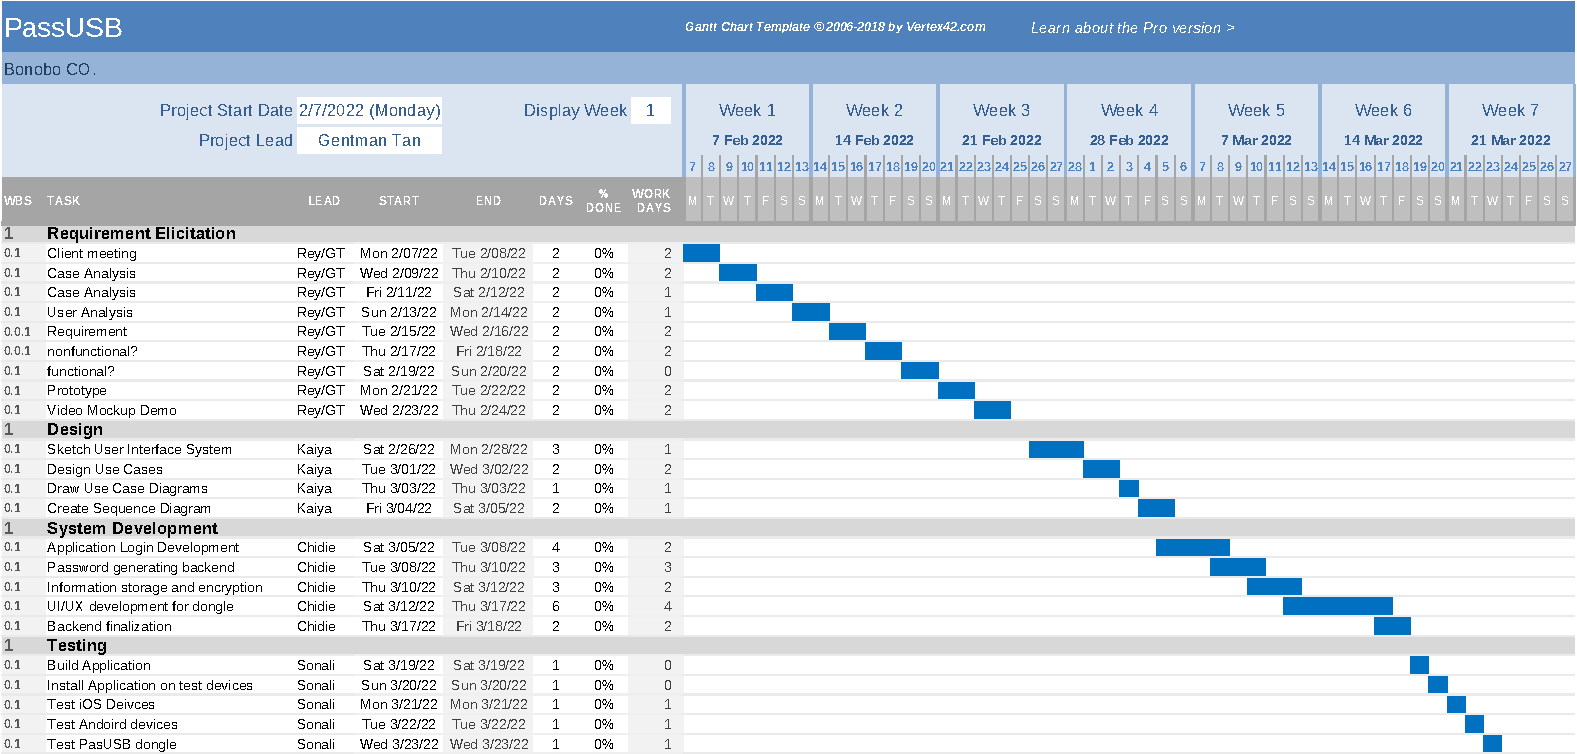
\includegraphics[scale=0.65]{ganttchart.pdf}

\section{Requirements Elicitation}

\subsection{Use Cases}

\scriptsize{\begin{xltabular}{\textwidth}{|l|X|}
  \hline Use Case ID: & UC-1-AA \\ \hline

  Use Case Name: & Add account \\ \hline

  Created By: Rey Jairus Marasigan & Last Updated By: Rey Jairus Marasigan \\ \hline

  Date Created: February 21, 2022 & Last Revision Date: February 21, 2022 \\ \hline

  Actors: & \nextitem User \\ \hline

  Description: &  This use case is used for specifying the different elements of our system that the DeviceUser goes through to add an entry to a list of account entries within our app. The ideal outcome of this use case is that the account is added to the database without any adverse effects. \\ \hline

  Trigger: & The user presses the plus icon on the top right of the UI. \\ \hline

  Preconditions: & \nextitem The User has created a database \nextitem The User has opened the app and unlocked their database \nextitem The User is in the correct directory to be able to see and touch the plus icon. \\ \hline

  Postconditions: & \nextitem At minimum: the system retains consistency and integrity in case of an error or deviation from the flow of events i.e. the user can “add account” again without repercussions from previous try.
    \nextitem Everything in harmony and works without error: Account is added to the database.
    \nextitem The account added can be accessed after being saved to the database. \\ \hline

  Normal Flow: & 
  (assumes the user wants to generate password when adding the account)
  \begin{enumerate}
    \item The DeviceUser presses the plus icon on the top right
    \item The view switches to a display that shows 3 text fields: a website field, a username and a password field. The first two will be required to be filled using the pop-up keyboard. The password field can either be manually filled or automatically generated using the associated button located to its left. <generate password use case>
    \item The user presses a button that opens to another view that shows multiple fields, boxes, and sliders to be filled, checked, and adjusted, respectively, to meet a certain criteria associated with the password.
    \item The user enters the field with a pop-up keyboard on their phone.
    \item Below the fields, the users checks various boxes or switches that configures the password generated by the apps such as:
      \nextitem contains special characters- an option that includes special characters in the password
      \nextitem contains numbers- an option that includes number
      \nextitem etc.
  \item Below the switches, there exists a slider that controls how long the password will be. When it is adjusted towards the right, it increases the length. When it is adjusted towards the left, it decreases the length. The maximum length of the slider occupies the entire width of the screen with some deadzone. The minimum length is 8 characters and the maximum is 32 characters. Initially the slider is set to 12.
  \item As the user changes the length of the desired password, a text box that shows the password itself changes. The password is shown in its pure form i.e. the actual password to be used. Here, the password is changeable by pressing on the box and using the pop-up keyboard. Initially, the password generated here is from the combination of the slider and checkboxes.
  \item The user then presses the "save password" button below to generate the password. <generate password use case>
  \item The user finally then presses the “add account” button below to add the account to the list.
  \item A notification pops up that lets the user know that the account has been added.
  \item The state of the app then returns to its default view.
  \end{enumerate} \\ \hline

 Alternative Flows: & \nextitemblank 2b. In step 2 of the normal flow, if the user chooses to manually enter the password rather than generate a new password,
   \begin{enumerate}
     \item The entire normal flow can skip to step 9
   \end{enumerate}
   \nextitemblank 7b. In step 7 of the normal flow, if the user changes the generated password and then slides the password slider,
   \begin{enumerate}
     \item An entirely different password is generated.
     \item The new password is instantly displayed within the text box.
     \item The normal use case continues thereafter on step 7 where the user can edit the newly generated password.
   \end{enumerate}
   \nextitemblank 9b. In step 9 of the normal flow, if the website field and username field is not filled
     \begin{enumerate}
     \item A notification pops up to let the user know about the required fields
     \item The app is scrolled the field needed to be filled
     \item The fields are highlighted red to indicate requirement. 
     \item The keyboard pops up automatically
     \item Once the fields are filled, the use case enters step 8 of the normal flow.
     \end{enumerate} \\ \hline

   Exceptions: & Exceptions to adding account to list
     \nextitemblank 9b. In step 9 of the normal flow, if the user does not enter a website or username. \\ \hline

   Includes: & editAccount- steps 3 to 7 would be required to edit an entry within the list and can be separated in its own use case \\ \hline

   Frequency of Use: & On-demand\\ \hline

   Special Requirements: & \nextitem Users should not wait >20 seconds for an action to be performed
     \nextitem Animations should last <250ms
     \nextitem Colors should be made to be accessible to colorblind
     \nextitem Application should be made available on all major mobile platforms \\ \hline


   Assumptions: & \nextitem The Customer has installed and is using the application
     \nextitem The application is readable to the Customer
     \nextitem The client has the ability to use the keyboard and interact with the screen. \\ \hline

   Notes and Issues: & \nextitem Is the minimum and maximum possible length of the password generator feasible for the users?
     \nextitem Should there be a limit to the amount of accounts added to the list?
     \nextitem What are the different switches that we can include in the forum?
     \nextitem should the app request for the master password (the password required to enter the app)or other biometrics for the ability to add an entry to the list?
     \nextitem Should we use other characters outside of the printable ascii characters? \\ \hline
\end{xltabular}}

\pagebreak

\scriptsize{\begin{xltabular}{\textwidth}{|l|X|}
  \hline Use Case ID: & UC-2-AB \\ \hline

  Use Case Name: & Login to Database \\ \hline

  Created By: Sonali Benni & Last Updated By: Sonali Benni \\ \hline

  Date Created: February 22, 2022 & Last Revision Date: February 22, 2022 \\ \hline

  Actors: & \nextitem DeviceUser \\ \hline
  
  Description: & This use case is for logging into the app to access passwords. Ideally, the actor would have the app on their phone. They would log into the app and have access to their home screen/ main menu. \\ \hline

  Trigger: & The DeviceUser clicks on the app on their personal device. \\ \hline

  Preconditions: & \nextitem The DeviceUser is logged in on their personal device such as a cellphone where the app is located. \nextitem The DeviceUser opens the app \\ \hline

  Postconditions: & \nextitem The DeviceUser is able to get into the app and is brought to a screen that allows them to enter login information.
    \nextitem The DeviceUser has successfully entered their information and is brought to a screen that shows their home screen.  \\ \hline

  Normal Flow: & 
    \begin{enumerate}
      \item The user turns on their personal device and is logged in. 
      \item The user then locates the app on their device. 
      \item The user clicks on the app.
      \item The app then opens and displays a login screen.
      \item The user then enters a username and password into the app.
      \item The information is successfully processed and the user can see their home screen.
      \item From this point, the user is free to update, add, or delete any accounts.
    \end{enumerate} \\ \hline

  Alternative Flows: & \nextitemblank 6a. In step 6 of the normal flow, the login information is not successfully processed and the user can’t see their home screen.
   \begin{enumerate}
      \item The app will prompt the user with an error, try again message 
      \item Once the information is correct and processed, the user is able to log in
      \item Use Case resumes on step 6
    \end{enumerate}
    \nextitemblank 7a. Once the user is successfully in the app, if the personal device were to turn off/shut down/force closed:
    \begin{enumerate}
      \item The user would be automatically signed out of the app.
      \item Use Case resumes on step 4 
   \end{enumerate} \\ \hline
  
  Exceptions: & \nextitemblank 4a. In step 4 of the normal flow, the login screen is not displaying 
    \begin{enumerate}
      \item If the app is down for maintenance or needs to be updated, a message will be displayed when the app is clicked on.
    \end{enumerate} 
  \nextitemblank 5a. The user forgets their password 
    \begin{enumerate}
      \item The user hits forget password
      \item Then a recovery key could be entered or security questions could be answered to login
      \item User is prompted to create a new password 
    \end{enumerate} \\ \hline

  Includes: &  Included in any Login use case scenarios \\ \hline

  Frequency of Use: & On-demand: Depends on how many accounts the user needs to login into on that particular day. This use case will most likely be used multiple times a day. \\ \hline

  Special Requirements: & The app should be organized and users should be able to quickly find what they are looking for. Color themes matter, color affects readability. \\ \hline

  Assumptions: & \nextitem The user understands English and knows their username and password for the app. \\ \hline

  Notes and Issues: & \nextitem Should the app have the ability to use Face ID or any other form of biometric authentication? \\ \hline

\end{xltabular}}

\pagebreak

\scriptsize{\begin{xltabular}{\textwidth}{|l|X|}
  \hline Use Case ID: & UC-232-AB \\ \hline

  Use Case Name: & Pair Dongle \\ \hline

  Created By: Gentman Tan & Last Updated By: Gentman Tan\\ \hline

  Date Created: February 22, 2022 & Last Revision Date: February 22, 2022 \\ \hline

  Actors: & \nextitem DeviceUser 
    \nextitem Mobile Device
    \nextitem PassUSB \\ \hline
  
  Description: &  Initialize a secure connection between the DeviceUser’s MobileDevice to the PassUSB for future device communication. \\ \hline

  Trigger: &  The DeviceUser initializes the pairing subroutine \\ \hline

  Preconditions: & \nextitem The DeviceUser is logged in on their personal device such as a cellphone where the app is located \nextitem The DeviceUser has the app opened \nextitem The DeviceUser has created a database \nextitem The DeviceUser has logged into a database \\ \hline

  Postconditions: & \nextitem The DeviceUser has successfully paired the PassUSB dongle to their database  \\ \hline

  Normal Flow: & 
    \begin{enumerate}
      \item The DeviceUser selects the "Pair Dongle" option in the drop down menu
      \item AccountHolder is prompted to enable bluetooth discovery mode
      \item The app searches for a PassUSB dongle
      \item Once found, the Bluetooth dongle's name, serial number and PIN number is displayed
      \item AccountHolder is prompted to either allow or decline the pairing process
      \item Once the AccoutHolder presses "Allow", they are prompted to enter the PIN number displayed on the PassUSB
      \item Once the PIN number is entered and confirmed, the devices are subsequently paired
    \end{enumerate} \\ \hline

  Alternative Flows: & 1a. In step 1 of the normal flow, a Bluetooth dongle is already paired 
    \begin{enumerate}
      \item The app will prompt the user to either unpair the already paired dongle or cancel the pairing process
      \item If the unpair button is pressed, the currently paired dongle is unpaired and PairDongle resumes on step 2
      \item If the cancel button is pressed, the pairing dialog box is closed and the PairDongle use case exits
    \end{enumerate} \\ \hline
  Exceptions: & \nextitemblank 3a. In step 3 of the normal flow, a Bluetooth dongle is not found  
    \begin{enumerate}
      \item The app will prompt the user to either retry or cancel the pairing process 
      \item If the retry button is selected, PairDongle resumes on step 3 
      \item If the cancel button is pressed, the pairing dialog box is closed and the PairDongle use case exits
    \end{enumerate} \\ \hline

  Includes: & N/A \\ \hline

  Frequency of Use: & On-demand \\ \hline

  Special Requirements: & \nextitem The app should filter out other unrelated Bluetooth devices that are discovered \\ \hline

  Assumptions: & \nextitem The DeviceUser understands English and knows their username and password for the app. \nextitem The DeviceUser has a funcitonal and powered PassUSB dongle \\ \hline

  Notes and Issues: & \nextitem Should the user have the ability to pair multiple different PassUSB dongles simultaneously? \\ \hline

\end{xltabular}}

\pagebreak

\scriptsize{\begin{xltabular}{\textwidth}{|l|X|}
  \hline Use Case ID: & UC-3-AC \\ \hline

  Use Case Name: & Generate Password \\ \hline

  Created By: Kaiya Roberts & Last Updated By: Kaiya Roberts \\ \hline

  Date Created: February 22, 2022 & Last Revision Date: February 22, 2022 \\ \hline

  Actors: & \nextitem DeviceUser \\ \hline
  
  Description: &  The reason behind this use case is to prevent the user from having to re use the same password or a variation of one combination of password. The ideal outcome of this use case will be the creation of a unique password with the requested character amount, letter amount, number amount, and special character amount. \\ \hline

  Trigger: & The user clicks on the create new password button on their personal device \\ \hline

  Preconditions: & \nextitem The DeviceUser is logged in on their personal device such as a cellphone where the app is located \nextitem The DeviceUser has the app opened \nextitem The DeviceUser has created a database \nextitem The DeviceUser has logged into a database \\ \hline

  Postconditions: & \nextitem The account holder has decided to not generate a password, but include their own password instead. Their own password will be stored in the account, and the account holder will be alerted that their password was stored \nextitem The password is generated with the conditions specifed by the accountHolder, and the accountHolder will be notified that the password was successfully created and it is stored into the system.  \\ \hline

  Normal Flow: & 
    \begin{enumerate}[nosep,after=\strut]
      \item The user has added the desired account that they would like to generate a password for (mentioned in the Add Account use case).
      \item The user has pressed the create a password button for the desired account. 
      \item The user device switches to a view where they have the option to click an eye icon that will show the password as it generates. 
      \item On the same view mentioned above the user has the option to choose between certain parameters that they can adjust based on the parameters of the password they would like to generate.
      \item The user clicks the parameter they would like to add to the password. The examples are provided below. 
        \begin{itemize}
          \item length of password
          \item upperCase letters 
          \item lowerCase letters
          \item digits
          \item Minus
          \item underscore
          \item space
          \item special characters
          \item bracket variations 
        \end{itemize}
    \item The user adjusts the desired length of password by moving the slider icon to their desired amount. 
      \begin{itemize}
          \item The slider starts at 12 characters and it can be adjusted to another number.
          \item The maximum number of characters in the password is 32. 
          \item When the slider is moved towards the right it increases the desired number
          \item When the slider moves towards the left it decreases the desired number
      \end{itemize}
    \item As the parameters are updated, the user will see the changes in the password box where the new password will be generated.
    \item The user updates the password with the desired parameters and has created a final password
    \item The user presses save password
    \item The password is saved into the application's database
    \end{enumerate} \\ \hline

  Alternative Flows: & \nextitem At any time, the user can cancel the Generate Password dialog box and exit the Generate Password use case \\ \hline

  Exceptions: & N/A \\ \hline

  Includes: & N/A \\ \hline

  Frequency of Use: & On-demand \\ \hline

  Special Requirements: & \nextitem Options chosen should reflect immediately in the password (the DeviceUser should not need to wait >500ms for a password to be generated) \\ \hline

  Assumptions: & \nextitem The DeviceUser understands English and knows their username and password for the app \nextitem The DeviceUser is logged into a database \nextitem The DeviceUser has elected to either add a new account entry or edit an existing account entry \\ \hline

  Notes and Issues: & \nextitem Which kinds of cryptographic algorithms should be used in the process of password generation? \nextitem Should passwords be shown in plaintext to the DeviceUser by default? \\ \hline

\end{xltabular}}

\pagebreak

\scriptsize{\begin{xltabular}{\textwidth}{|l|X|}
  \hline Use Case ID: & UC-5-AC \\ \hline

  Use Case Name: & Delete Account \\ \hline

  Created By: Chidiebere Otuonye & Last Updated By: Chidiebere Otuonye \\ \hline

  Date Created: February 21, 2022 & Last Revision Date: February 22, 2022 \\ \hline

  Actors: & \nextitem DeviceUser \\ \hline
  
  Description: & This use case is for outlining the behavior of DeviceUser when they’re deleting an account from the USB dongle, via the app.\\ \hline

  Trigger: & The user presses the “edit” button. \\ \hline

  Preconditions: & \nextitem The DeviceUser is logged in on their personal device such as a cellphone where the app is located \nextitem The DeviceUser has the app opened \nextitem The DeviceUser has created a database \nextitem The DeviceUser has logged into a database \\ \hline

  Postconditions: & \nextitem The system retains all data from accounts that user intends to keep and integrity of control flow is preserved \nextitem The correct account is deleted and the other accounts are preserved, control flow is preserved and the user can execute other actions and navigate to other parts of app  \\ \hline

  Normal Flow: & 
    \begin{enumerate}
      \item The accountHolder presses the 'edit' icon.
      \item Selection bubbles appear next to all accounts.
      \item The accountholder can select multiple accounts or just 1.
      \item The accountholder selects the trash icon in the top right-hand corner.
      \item A dialogue box pops up asking if user is sure they want to delete selected accounts.
      \item App authenticates identity before deleting account.
    \end{enumerate} \\ \hline

  Alternative Flows: & 
    \nextitemblank 3a. In step 3 the user decides not to delete any accounts after pressing 'edit'.
      \begin{enumerate}
        \item User selects 'cancel' in top left-hand corner where the 'edit' button previously was.
        \item Selection bubbles disappear from next to account fields.
      \end{enumerate}
    \nextitemblank 3b. In step 3 the user decides not to delete any accounts after pressing 'edit' and selecting account(s).  
      \begin{enumerate}
        \item User selects 'cancel' in top left-hand corner where the 'edit' button previously was.
        \item Selection bubbles disappear from next to account fields.
      \end{enumerate}
    \nextitemblank 3c. In step 3 the user decides to delete all accounts after pressing 'edit' button.
      \begin{enumerate}
        \item User presses the 'select all' button.
        \item User presses the trash icon.
        \item User is prompted to confirm if they're sure they want to delete 'ALL accounts'.
        \item User is prompted to authenticate using physical password.
        \item User is then prompted once more if they'd like to delete 'ALL accounts as the action is irreversible'
        \item User selects 'delete' and all accounts are deleted.
      \end{enumerate}
    \nextitemblank 5a. In step 5 user decides not to delete accounts after selecting the trash icon.
      \begin{enumerate}
        \item User selects the 'Never mind' option when presented with the options to delete or not delete selected accounts. 
      \end{enumerate} \\ \hline

  Exceptions: & 
    \nextitemblank 6a. In step 6 user isn't able or chooses not to authenticate their identity to complete deletion process.
      \begin{enumerate}
      \item User fails authentication and is prompted to authenticate biometrically 2 additional times.
      \item User is then asked to enter physical password.
      \item User enters physical password incorrectly 3 times and is locked out of account for 30 minutes.
      \item User enters physical password incorrectly 1 more time and is locked out for 45 minutes.
      \item User enters physical password incorrectly 1 more time and is locked out for 1 hour.
      \item User enters physical password incorrectly 1 more time and is locked out permanently until they recover account. N/A 
      \end{enumerate} \\ \hline
  Includes: & N/A \\ \hline

  Frequency of Use: & On-demand \\ \hline

  Special Requirements: & \nextitem Customer can organize accounts with different methods to make deleting quicker. \\ \hline

  Assumptions: & \nextitem The user is able to use the application without issue on their device(s). \nextitem The user understands which button to choose to select and delete accounts \\ \hline

  Notes and Issues: & \nextitem Should account objects that are to be deleted undergo lazy deletion or completely dereferenced? \\ \hline

\end{xltabular}}

% BEGIN PART 2

\scriptsize{\begin{xltabular}{\textwidth}{|l|X|}
  \hline Use Case ID: & UC-6-AC \\ \hline

  Use Case Name: & Backup Database \\ \hline

  Created By: Gentman Tan & Last Updated By: Gentman Tan\\ \hline

  Date Created: April 9, 2022 & Last Revision Date: April 9, 2022 \\ \hline

  Actors: & \nextitem DeviceUser \nextitem FlashDrive  \\ \hline

  Description: & This use case specifies the process of which a database is backed up onto an external storage device \\ \hline

  Trigger: & The DeviceUser presses the 'backup' button. \\ \hline

  Preconditions: & \nextitem The DeviceUser is logged in on their personal device such as a cellphone where the app is located \nextitem The DeviceUser has the app opened \nextitem The DeviceUser has created a database \nextitem The DeviceUser has logged into a database \\ \hline

  Postconditions: & \nextitem An encrypted container containing the database is created on a user selected external storage device  \\ \hline

  Normal Flow: &
    \begin{enumerate}
      \item The DeviceUser presses the 'backup' menu entry.
      \item The DeviceUser is shown a system directory chooser and is prompted to select a directory to be used to save the database backup
      \item The DeviceUser chooses a directory
      \item The DeviceUser receives confirmation that the account database is backed up onto the specified directory with the filename passusb-<date>.bak, where <date> would be in the format MMDDYYYY, for example 01012001 for January 1, 2001.
    \end{enumerate} \\ \hline

  Alternative Flows: &
                       \nextitemblank 3a. In step 3, a file of the same name as the backup file already exists
                       \begin{enumerate}
                               \item The DeviceUser is prompted that a file of the same name as the new backup
                               \item The DeviceUser chooses to either overwrite the file, rename the new file backup file or cancel the backup procedure
                       \end{enumerate}
                       

              \\ \hline

  Exceptions: &
                \nextitemblank 3b. In step 3, the directory is unwriteable
                       \begin{enumerate}
                               \item The DeviceUser is prompted that the directory that has been chosen is invalid and is presented the corresponding error (for example, directory is read only)
                               \item The DeviceUser is presented with the options to either choose a new directory or cancel the backup procedure
                       \end{enumerate}
              \\ \hline
  Includes: & N/A \\ \hline

  Frequency of Use: & On-demand \\ \hline

  Special Requirements: & \nextitem The backup file should be resilient to data corruption \\ \hline

  Assumptions: & \nextitem The DeviceUser is able to use the application without issue on their device(s). \nextitem The DeviceUser understands which button to choose to backup the database \nextitem The DeviceUser uses a storage medium with a filesystem that is supported by the mobile operating system. \\ \hline

  Notes and Issues: & N/A \\ \hline

\end{xltabular}

\scriptsize{\begin{xltabular}{\textwidth}{|l|X|}
  \hline Use Case ID: & UC-6-AC \\ \hline

  Use Case Name: & Create account entry group \\ \hline

  Created By: Gentman Tan & Last Updated By: Gentman Tan\\ \hline

  Date Created: April 9, 2022 & Last Revision Date: April 9, 2022 \\ \hline

  Actors: & \nextitem DeviceUser \\ \hline

  Description: & This use case specifies the process of which an account entry is grouped \\ \hline

  Trigger: & The DeviceUser presses the 'add group' button. \\ \hline

  Preconditions: & \nextitem The DeviceUser is logged in on their personal device such as a cellphone where the app is located \nextitem The DeviceUser has the app opened \nextitem The DeviceUser has created a database \nextitem The DeviceUser has logged into a database \\ \hline

  Postconditions: & \nextitem An account entry group is created \\ \hline

  Normal Flow: &
    \begin{enumerate}
            \item The DeviceUser presses the 'add group' button
            \item A new list entry is presented in the account list view section of the app with a folder icon and text entry field for the user to create a new name for the account group
            \item The DeviceUser types in an appropriate name for the account group
            \item The DeviceUser presses return on their keyboard and the account group is created

    \end{enumerate} \\ \hline

  Alternative Flows: &
                       \nextitemblank 3a. In step 3, the user does not input any characters for a name for the folder
                       \begin{enumerate}
                               \item The DeviceUser presses retur no ntheir keyboard and an account group with the name ``New Folder'' is created. If a folder exists with this name, a number will be appended to the name i.e. ``New Folder (<number>)''
                       \end{enumerate}
              \\ \hline

  Exceptions: &
                N/A
              \\ \hline
  Includes: & N/A \\ \hline

  Frequency of Use: & On-demand \\ \hline

  Special Requirements: & \nextitem The backup file should be resilient to data corruption \\ \hline

  Assumptions: & \nextitem The DeviceUser is able to use the application without issue on their device(s). \nextitem The DeviceUser understands which button to choose to create an account group \\ \hline

  Notes and Issues: & N/A \\ \hline

\end{xltabular}

\subsection{Use Case Diagrams}

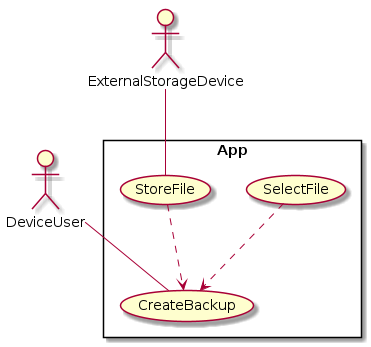
\includegraphics[scale=0.5]{diag/gt/uc1.png}

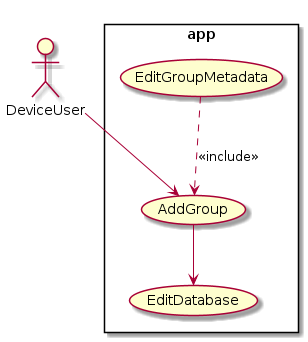
\includegraphics[scale=0.5]{diag/gt/uc2.png}

\section{Reqirements Analysis}

\subsection{Scenarios}

\subsection{Static model}

\subsubsection{Object Diagrams}

\subsubsection{Class Diagram}

\subsection{Dynamic Model}

%\section{Glossary}
%
%\pagebreak
%
%\section{Approval Page}
%
%\pagebreak
%
%\section{References}

%\pagebreak
%
%\section{Appendix}
%
%\subsection{Diary of meeting and tasks}
%
%$Monday the 31st from 6:15 to 7:20:
%\nextitem Our group met today for about an hour to discuss project ideas. We picked a project and completed the project proposal. 
%
%$Wednesday the 9th from 6:15 to 7:00:
%\nextitem Our group met today for about an hour to complete the in-class assignment. 
%
%$Monday the 14th from 6:15 to 7:15:
%\nextitem Our group met today to discuss the Group Project Part I: Analysis. We assigned roles and discussed how to go forward with the execution of the rest of the project. 
%
%$Wednesday the 16th from 6:15 to 7:00:
%\nextitem Our group met today to complete the third in-class activity. 
%
%$Monday the 21st from 5:10 to 6:15:
%\nextitem Our group met today in class and worked on our use cases for our project.
%
%$Monday 28th of March from 6:10 to 6:30
%\nextitem We discussed Analysis 2 and assigned tasks
%
%$Wednesday the 30th of March from 5:45 to 6:15:
%\nextitem We completed the in-class activity
%
%$Wednesday the 6th of April from 5:50 to 7:30:
%\nextitem We completed the in-class activity
%
%$Wednesday the 13th of April from 5:50 to 7:00:
%\nextitem We worked on the diagrams for the project


\end{document}
%% 
%% Copyright (C) 2021 by Daniel A. Weiss <daniel.weiss.led at gmail.com>
%% 
%% This work may be distributed and/or modified under the
%% conditions of the LaTeX Project Public License (LPPL), either
%% version 1.3c of this license or (at your option) any later
%% version.  The latest version of this license is in the file:
%% 
%% http://www.latex-project.org/lppl.txt
%% 
%% Users may freely modify these files without permission, as long as the
%% copyright line and this statement are maintained intact.
%% 
%% This work is not endorsed by, affiliated with, or probably even known
%% by, the American Psychological Association.
%% 
%% 
%% This work is "maintained" (as per LPPL maintenance status) by
%% Daniel A. Weiss.
%% 
%% This work consists of the file  apa7.dtx
%% and the derived files           apa7.ins,
%%                                 apa7.cls,
%%                                 apa7.pdf,
%%                                 README,
%%                                 APA7american.txt,
%%                                 APA7british.txt,
%%                                 APA7dutch.txt,
%%                                 APA7english.txt,
%%                                 APA7french.txt,
%%                                 APA7german.txt,
%%                                 APA7ngerman.txt,
%%                                 APA7greek.txt,
%%                                 APA7czech.txt,
%%                                 APA7turkish.txt,
%%                                 APA7endfloat.cfg,
%%                                 Figure1.pdf,
%%                                 shortsample.tex,
%%                                 longsample.tex, and
%%                                 bibliography.bib.
%% 
%%
%% End of file `./samples/longsample.tex'.
